\chapter{Problemanalyse}
\textit{I dette kapitel analyses problemstillinger, som opstår i forbindelse med lægemiddelskift. Disse problemstillinger vil sammenfattes i en opsummering og afsluttes med en problemformulering, der fremadrettet danner  grundlaget for rapporten.}

\section{Årsager til lægemiddelskift}
Lægemiddelskift kan forekomme i forbindelse med kontraktskift, restordre eller bagatelkøb~\citep{Amgros2015}. Kontraktskift kan forekomme ved at lægemidlerne sendes i udbud, såkaldt amgrosudbud. Udbuddene forekommer hvis der findes mere end én leverandør af lægemidlet. Lægemidlerne bringes derved i konkurrence, hvilket kan give anledning til kontraktskift. I tilfælde af patent på lægemidlet, hvormed der kun findes én leverandør, er der ofte ikke konkurrence, da prisen på lægemidlet allerede er fastsat.~\citep{Amgros2015} 

Restordre forekommer når efterspørgslen på et lægemiddel overstiger den tilgængelige mængde.~\citep{Amgros2015}. Dette kan ske ved f.eks. leveringesvigt fra leverandøren eller producenten på det ønskede lægemiddel~\citep{Amgros2017, Laegemiddelinformaion2017}. Leveringesvigt skyldes som ofte at producenten har mangel på råvarer eller produktionsvanskeligheder.~\citep{Amgros2017, Laegemiddelinformaion2017} 

%I tilfælde af restordre er det leverandørens ansvar at dække hospitalsapotekernes udgift ved indkøb af et erstatningslægemiddel~\fxnote{\url{https://levportal.amgros.dk/SiteCollectionDocuments/1.\%20Grundl\%C3\%A6ggende\%20information\%20om\%20l\%C3\%A6gemiddeludbud.pdf}}.
 
En gang årligt i maj/juni publiceres bagatelkøb af amgros, hvilket kan forårsage lægemiddelskift~\citep{Amgros2018}. I disse tilfælde modtager Amgros pristilbud fra leverandørere med henblik på økonomisk besparelser på lægemiddlerne, hvilket kan føre til lægemiddelskift~\citep{Amgros2012}. 

%I disse tilfælde er sygehusapoteket ikke forpligtet til at anvende lægemidlet og leverandøren omfattes ikke af indkøbs- eller forsyningspligt.~\citep{Amgros2018}Amgros publicerer hvert år i maj/juni udbud for en række lægemidler med en mindre omsætning, der ligger under tærskelværdierne, men som kan have grænseoverskridende interesse. Derfor udbyder vi disse indkøb efter reglerne for udbud under tærskelværdierne. Det er derudover muligt for leverandører at afgive løbende tilbud på de ATC-koder, der er omfattet af bagatelkøb.

\subsection{Kontraktskift}
Før et muligt kontraktskift kan finde sted og udbud på lægemidler sker har Amgros en dialog med medicinrådet~\citep{Amgros2017, Amgros2017a}. Lægemidlerne vurderes i forhold til effekt, eksisterende behandling og pris med det formål at stræbe efter laveste priser samt bedst mulig behandling for patienterne. Medicinrådet kategoriserer nye lægemidler og indikationer i forhold til den nuværende standardbehandling i stor, vigtig, lille eller ingen merværdi. Ud fra dette sammenstiller Amgros standardbehandlingen over for en omkostningsanalyse, der er udarbejdet af ansøgeren for lægemiddelskift. Amgros vurderer, hvorvidt de tilsendte oplysninger er relevante og valide. Den kliniske merværdi, omkostningsanalyse og estimeringen af budget konsekvenser danner grundlaget for prisforhandling. Medicinrådet beslutter efter prisforhandlingen, hvorvidt det nye lægemiddel skal anvendes som standardbehandling. Hvis dette er tilfældet foretages et kontraktskift.~\citep{Amgros2017, Amgros2017a}

\subsection{Restordre}
Restordre kan kategoriseres som simpel eller kompleks i forhold til hvordan de påvirker klinikken~\citep{Laegemiddelinformaion2017}. En simpel restordre er vurderet til at påvirke klinikken i lav grad. Disse opstår dagligt når et lægemiddel skiftes til en simpel generiske lægemiddel og varetages ofte af sygehusapotekets logistik-afdeling. ~\citep{Laegemiddelinformaion2017}

En kompleks restordre vurderes til at påvirke klinikken i mellem til høj grad ~\citep{Laegemiddelinformaion2017}. Disse sker i forbindelse med mere kompleks skift til generiske lægemidler i forbindelse med ændringer af f.eks. styrke, disponeringsform  og andre hjælpestoffer. I tilfælde af kompleks restordre henvendes der ofte til den medicinansvarlige, kontraktsygeplejersker eller medicinservicefarmakonomerne i forhold til at undersøge om lægemidlet er anvendeligt for det pågældende hospitalsafsnit. Hensigten i tilfælde af komplekse restordre er at finde en erstatning i god tid, at erstatning ligner det lægemiddel der er i restordre samt mindske ændringer ved klinikkens arbejdsgang.~\citep{Laegemiddelinformaion2017}

Der udføres en faglig risikovurdering i samarbejde med sygehusapoteket og eventuelt i samarbejde klinikken ved restordre ~\citep{Laegemiddelinformaion2017}. Dette gøres med henblik på optimal lægemiddelbehandling i forhold til patientsikkerhed, ændringer i håndtering og opbevaringsbetingelser af lægemidlet. Erstatningslægemidlet vurderes ud fra prioriteringen registeret specialitet (RS), ikke-registeret specialist (IRS) og magistrelt lægemiddel~\citep{Laegemiddelinformaion2017}.


\section{Problematikker ved lægemiddelskift}
Der er både økonomiske og patientsikkerhedsmæssige konsekvenser ved et lægemiddelskift for så vidt angår restordre såvel som kontraktskift~\citep{Amgros2015}. Restordre er økonomisk omkostningsfuldt, da der skal foretages vareskift i systemer, på lagre og i medicinrum. Yderligere skal der gives behandlingsinstruktioner til hospitalsafdelingerne for at undgå fejl ved medicinering. Udover økonomiske faktorer udgør lægemiddelskift også patientsikkerhedsmæssige risici. Der kan opstå utilsigtede hændelser (UTH'er), hvis præparatet har skiftet navn, udseende og håndteringen af medicin er ændret.~\citep{Amgros2015}. 

De hyppigste årsager til UTH'er på de danske hospitaler skyldes i år 2013, 23,97~\%,medicinering, 20,86~\% kliniske processor, 17,98~\% kommunikation og dokumentation samt 17,23~\% administrative processer~\citep{Patientombuddet2013}. Antallet af rapporterede UTH'er i Region Nordjylland er steget med over 36\% fra år 2012 til 2014 ~\citep{Jensen2014}. Ud af 824 rapporterede UTH'er i år 2014 omhandlede 97\% medicinering, 86\% administration af medicin og 41\% at medicinen ikke var givet~\citep{Jensen2014}. 

\subsection{Kontraktskift}
De patientsikkerhedsmæssige konsekvenser opstået ved kontraktskift er undersøgt af et norsk studie~\citep{Hakonsen2010}. Interview med 100 sygeplejersker påviste at der opstod fejlmedicinering ved generiske lægemidler. Fejl i ordination og manglende dokumentation af lægemiddelskiftet af lægen blev opdaget af 46~\% sygeplejersker dagligt, hvorimod sygeplejerskerne altid fik lægemiddelsiftet dokumenteret. Yderligere følte 92~\% af sygeplejerskerne at generiske lægemidler var tidskrævende og 91~\% at disse øgede risikoen for fejl ved disponering.~\citep{Hakonsen2010}. De typiske hændelser ved kontraktskift fremgår af Figur \ref{fig:UTHkontraktskift}.

\begin{figure}[H]\centering
	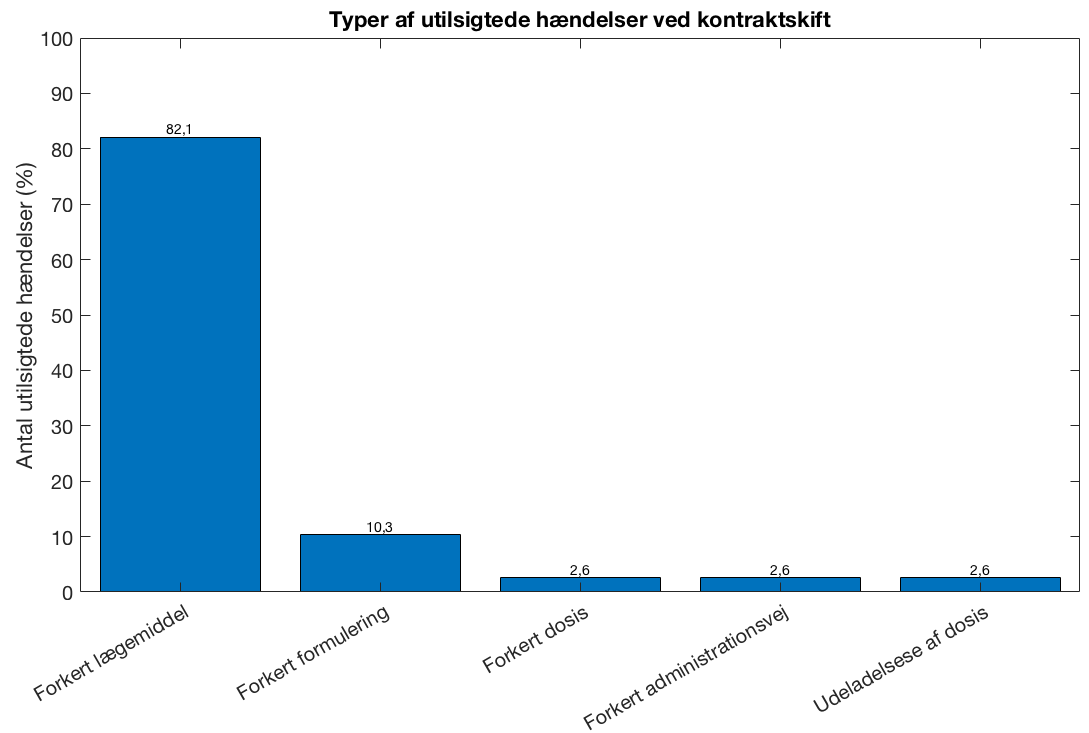
\includegraphics[width=0.7\textwidth]{billeder/UTH1.png} 
	\caption{Utilsigtede hændelser opstået ved kontraktskift\citep{Hakonsen2010}.}
	\label{fig:UTHkontraktskift}  
\end{figure}

Af Figur \ref{fig:UTHkontraktskift} fremgår det at 82,1~\% af UTH'erne forekommer ved disponering af forkert lægemiddel. Den næst hyppigste er forkert formulering \fxnote{hvad menes der med formulering?}


\subsection{Restordre}

*** KIG 3.5.5. Utilsigtede hændelser forårsaget af Restordre *** 16 PDF

De typiske hændelser ved restordre fremgår af Figur \ref{fig:UTHrestordre}.

\begin{figure}[H]\centering
	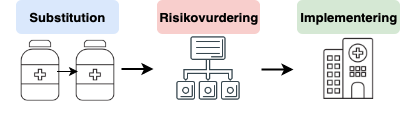
\includegraphics[width=1\textwidth]{billeder/forside.png} 
	\caption{Utilsigtede hændelser opstået ved restordre\citep{Hakonsen2010}.}
	\label{fig:UTHRestordre}  
\end{figure}


\section{Løsningsstartegier for problematikker}

\subsection{Kontraktskift}

\subsection{Restordre}
Disse risici kan mindskes ved instrukser og ændring af procedure på hospitalerne.
Tæt dialog med leverandøren.

*** SE 19Præparat ***

Jeg skal mere kigge på om det er muligt at gruppere de ting der skal gøres ved lægemiddelskift. Altså vejledninger. 


\section{Opsummering}
\subsection{Problemformulering}